%Chapter 3
\chapter{Developing a simulation methodology}
\thispagestyle{empty}
\vspace{38em}
\hrulefill
\\
\enquote*{\textit{Quote.}} - Somebody\\
\newpage
\section{Introduction}
\section{System investigation method}
	\subsection{Preamble}
		Developing a detailed simulation model of a compressed air network requires thorough comprehension of the inner workings of the system. This section will discuss the investigations needed to obtain the required understanding.
	\subsection{Data acquisition and verification} % 
		- Layouts, data from SCADA Instrumentation, etc.\\
		- Verification of accurate data - Gous article
	\subsection{Solutions to unavailable data}
		Parameters that are required to develop the simulation model, such as flows, pressures, may not be actively logged by mine systems. To obtain this data it is necessary to investigate alternative sources. At points where instrumentation is absent, estimations can be made from assumptions made using instrumentation on the network or spot inspections.
		\par 
		Air network specifications such as piping sizes, technical layouts, major leak locations or specifications is often outdated or not recorded. Critical data should be obtained through audits and inspections of the system. If manual inspection is not possible, estimations should be made using the available data or approximation techniques discussed in literature. \texttt{REMEMBER TO REFERENCE\\ SPECIFIC LOCATION LITERATURE}.
	\subsection{Mining schedule}
		A crucial aspect to developing an accurate model of a mining compressed air system is understanding the the operational philosophy of the mine. The schedule for operations such as drilling,  blasting or cleaning can have a major impact on compressed air requirements at different times of the day. By utilizing the operational schedule, simulation scenarios can be optimized for the air requirements throughout the day.
	\subsection{Summary}
\section{Model development and verification}
	\subsection{Preamble}
	Compressed air networks are comprised of components such as compressors, valves, pipes, etc. This section  the development of component models that make up a compressed air simulation is discusses. Verification methods is then discussed.
	\subsection{Compressed air component models}
		\subsubsection{Air pipes and valves}
		Pressure losses that occur due to pipe friction losses should be included for large piping sections in the simulation . A pipe component is used to account for these losses which are defined by the \textit{Darcy-Weisbach equation}\footnote{ B. Glenn, \enquote*{The Darcy–Weisbach Equation,}[Online] \url{https://bae.okstate.edu/faculty-sites/Darcy/DarcyWeisbach/Darcy-WeisbachEq.htm}, [Accessed 20-05-2017]}:
		$$\Delta P = \frac{f  L \rho V^2}{2 D}$$
		Where the pressure difference $\Delta P $ is a function of:\\
		\begin{tabular}{p{1.3cm}p{13cm}}
		$f$ & Friction coefficient  \\
		$L$ & Pipe length ($m$) \\
		$D$ & Pipe diameter ($m$) \\
		$\rho$ & Air density ($kg/m^3$)\\	
		$V$ & Average velocity ($m/s$) \\
		\end{tabular} \\
		The component model can be used as a valve by controlling the open fraction between 0 and 1. Modeling the valve flow characteristics is discussed in \ref{Controllers} \textit{Controllers}.
		\subsubsection{Ambient conditions}
		Ambient air condition underground and on surface can effect the performance of the network [\texttt{Citation needed}]. Pressure and temperature increases with depth as a result of auto compression and rock face temperature [\texttt{Citation needed}]. Therefore it is important to take into account conditions for the boundary conditions at each mining level or area where compressed air is used.   
		\paragraph{Compressors}\leavevmode\\
		Three compressor models were investigated, each with varying complexity. The models are: air compressor, dynamic compressor and positive displacement compressor. 
		\par 
		The air compressor model is a general, simplified compressor model. This model requires minimal user inputs by making several assumptions. This is useful when parameters for a compressor are not available. Or when doing a quick preliminary simulation. However it is not ideal for detailed simulations which require more precision. 
		\par 
		The dynamic and positive displacement compressor models are more complex, taking into account factors such as heat caused by polytopic compression and inefficiencies. The models do still make several assumptions for example, the compressor efficiency at different loads is assumed to remain the same. This can cause the operation of the model can differ slightly from the real life compressor.
		\par 	 
		For most scenarios, the dynamic compressor component is most suitable. This component is modeled by fitting a quadratic curve through three points of operation to obtain an equation for corrected mass flow as a function of the pressure ratio. This characteristic curve of compressor  as shown in figure \ref{fig: Compressor Curve} can be accurately estimated even when only one data point is available by making approximations for the zero flow and pressure points on the curve.
		\begin{figure}[h]
			\centering
			\fbox{% GNUPLOT: LaTeX picture with Postscript
\begingroup
  \makeatletter
  \providecommand\color[2][]{%
    \GenericError{(gnuplot) \space\space\space\@spaces}{%
      Package color not loaded in conjunction with
      terminal option `colourtext'%
    }{See the gnuplot documentation for explanation.%
    }{Either use 'blacktext' in gnuplot or load the package
      color.sty in LaTeX.}%
    \renewcommand\color[2][]{}%
  }%
  \providecommand\includegraphics[2][]{%
    \GenericError{(gnuplot) \space\space\space\@spaces}{%
      Package graphicx or graphics not loaded%
    }{See the gnuplot documentation for explanation.%
    }{The gnuplot epslatex terminal needs graphicx.sty or graphics.sty.}%
    \renewcommand\includegraphics[2][]{}%
  }%
  \providecommand\rotatebox[2]{#2}%
  \@ifundefined{ifGPcolor}{%
    \newif\ifGPcolor
    \GPcolortrue
  }{}%
  \@ifundefined{ifGPblacktext}{%
    \newif\ifGPblacktext
    \GPblacktextfalse
  }{}%
  % define a \g@addto@macro without @ in the name:
  \let\gplgaddtomacro\g@addto@macro
  % define empty templates for all commands taking text:
  \gdef\gplbacktext{}%
  \gdef\gplfronttext{}%
  \makeatother
  \ifGPblacktext
    % no textcolor at all
    \def\colorrgb#1{}%
    \def\colorgray#1{}%
  \else
    % gray or color?
    \ifGPcolor
      \def\colorrgb#1{\color[rgb]{#1}}%
      \def\colorgray#1{\color[gray]{#1}}%
      \expandafter\def\csname LTw\endcsname{\color{white}}%
      \expandafter\def\csname LTb\endcsname{\color{black}}%
      \expandafter\def\csname LTa\endcsname{\color{black}}%
      \expandafter\def\csname LT0\endcsname{\color[rgb]{1,0,0}}%
      \expandafter\def\csname LT1\endcsname{\color[rgb]{0,1,0}}%
      \expandafter\def\csname LT2\endcsname{\color[rgb]{0,0,1}}%
      \expandafter\def\csname LT3\endcsname{\color[rgb]{1,0,1}}%
      \expandafter\def\csname LT4\endcsname{\color[rgb]{0,1,1}}%
      \expandafter\def\csname LT5\endcsname{\color[rgb]{1,1,0}}%
      \expandafter\def\csname LT6\endcsname{\color[rgb]{0,0,0}}%
      \expandafter\def\csname LT7\endcsname{\color[rgb]{1,0.3,0}}%
      \expandafter\def\csname LT8\endcsname{\color[rgb]{0.5,0.5,0.5}}%
    \else
      % gray
      \def\colorrgb#1{\color{black}}%
      \def\colorgray#1{\color[gray]{#1}}%
      \expandafter\def\csname LTw\endcsname{\color{white}}%
      \expandafter\def\csname LTb\endcsname{\color{black}}%
      \expandafter\def\csname LTa\endcsname{\color{black}}%
      \expandafter\def\csname LT0\endcsname{\color{black}}%
      \expandafter\def\csname LT1\endcsname{\color{black}}%
      \expandafter\def\csname LT2\endcsname{\color{black}}%
      \expandafter\def\csname LT3\endcsname{\color{black}}%
      \expandafter\def\csname LT4\endcsname{\color{black}}%
      \expandafter\def\csname LT5\endcsname{\color{black}}%
      \expandafter\def\csname LT6\endcsname{\color{black}}%
      \expandafter\def\csname LT7\endcsname{\color{black}}%
      \expandafter\def\csname LT8\endcsname{\color{black}}%
    \fi
  \fi
    \setlength{\unitlength}{0.0500bp}%
    \ifx\gptboxheight\undefined%
      \newlength{\gptboxheight}%
      \newlength{\gptboxwidth}%
      \newsavebox{\gptboxtext}%
    \fi%
    \setlength{\fboxrule}{0.5pt}%
    \setlength{\fboxsep}{1pt}%
\begin{picture}(9360.00,4032.00)%
    \gplgaddtomacro\gplbacktext{%
      \colorrgb{0.00,0.00,0.00}%
      \put(814,704){\makebox(0,0)[r]{\strut{}$0$}}%
      \colorrgb{0.00,0.00,0.00}%
      \put(814,1261){\makebox(0,0)[r]{\strut{}$100$}}%
      \colorrgb{0.00,0.00,0.00}%
      \put(814,1818){\makebox(0,0)[r]{\strut{}$200$}}%
      \colorrgb{0.00,0.00,0.00}%
      \put(814,2375){\makebox(0,0)[r]{\strut{}$300$}}%
      \colorrgb{0.00,0.00,0.00}%
      \put(814,2932){\makebox(0,0)[r]{\strut{}$400$}}%
      \colorrgb{0.00,0.00,0.00}%
      \put(814,3489){\makebox(0,0)[r]{\strut{}$500$}}%
      \colorrgb{0.00,0.00,0.00}%
      \put(946,484){\makebox(0,0){\strut{}$0$}}%
      \colorrgb{0.00,0.00,0.00}%
      \put(1948,484){\makebox(0,0){\strut{}$2$}}%
      \colorrgb{0.00,0.00,0.00}%
      \put(2950,484){\makebox(0,0){\strut{}$4$}}%
      \colorrgb{0.00,0.00,0.00}%
      \put(3952,484){\makebox(0,0){\strut{}$6$}}%
      \colorrgb{0.00,0.00,0.00}%
      \put(4954,484){\makebox(0,0){\strut{}$8$}}%
      \colorrgb{0.00,0.00,0.00}%
      \put(5956,484){\makebox(0,0){\strut{}$10$}}%
      \colorrgb{0.00,0.00,0.00}%
      \put(6958,484){\makebox(0,0){\strut{}$12$}}%
      \colorrgb{0.00,0.00,0.00}%
      \put(7960,484){\makebox(0,0){\strut{}$14$}}%
      \colorrgb{0.00,0.00,0.00}%
      \put(8962,484){\makebox(0,0){\strut{}$16$}}%
      \csname LTb\endcsname%
      \put(5455,3043){\makebox(0,0)[l]{\strut{}$f(x) = -2.586x^2 + 7.788x + 494$}}%
    }%
    \gplgaddtomacro\gplfronttext{%
      \csname LTb\endcsname%
      \put(176,2235){\rotatebox{-270}{\makebox(0,0){\strut{}Mass flow ($kg^3/s/\sqrt(k)/Bar$)}}}%
      \put(4954,154){\makebox(0,0){\strut{}Pressure ratio}}%
    }%
    \gplbacktext
    \put(0,0){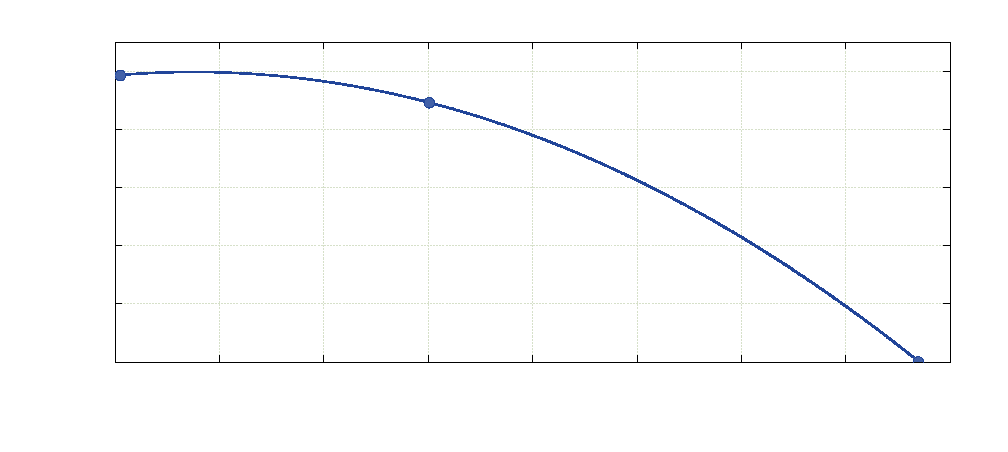
\includegraphics{Graphs/3/AproxCurve/AproxCurve}}%
    \gplfronttext
  \end{picture}%
\endgroup
}
			\caption{Estimating the characteristic curve of a compressor by fitting a quadratic function to points of operation.}
			\label{fig: Compressor Curve}
		\end{figure}
		\par
		Once accurately modeled, the compressor component is added to the air network in the arrangement shown in figure \ref{fig: Compressor models}. The Compressor is connected to the inlet air source via an inlet pipe and air node and to the rest of the network via an air node and outlet pipe. This is is to allow the inlet and outlet parameters and conditions to be be monitored and controlled.
		\begin{figure}[h]
			\centering
			\fbox{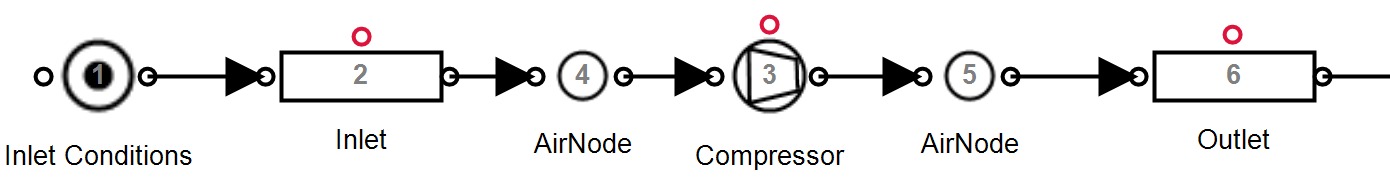
\includegraphics[trim =-4cm 0 -4cm 0cm, width=\textwidth]{Images/3/Compressors}}
			\caption{Integrating the compressor component into the simulation.}
			\label{fig: Compressor models}
		\end{figure}		

		\subsubsection{Demand/leak}
			A flow demand 
		\subsubsection{Controllers}\label{Controllers}
		Simulated components need to be dynamically controlled as in the actual air network. Typically compressors and valves are controlled to certain set-points and schedules. It is important to model the nonlinearities of these controllers to ensure the simulation reacts in the same way the actual network would.
		\par 
		On a typical mine, compressors power is controlled such that the discharge pressure matches a specified set-point. Power control is achieved through either \glspl{vsd} \slash \glspl{vfd} or guide-vain control. \glspl{vfd} provide a wide range of power control and can be estimated using a \gls{pi} controller as in figure \ref{fig: Controller models} where discharge pressure is used as feedback for the controller. 
	\begin{figure}[h]
		\centering
		\fbox{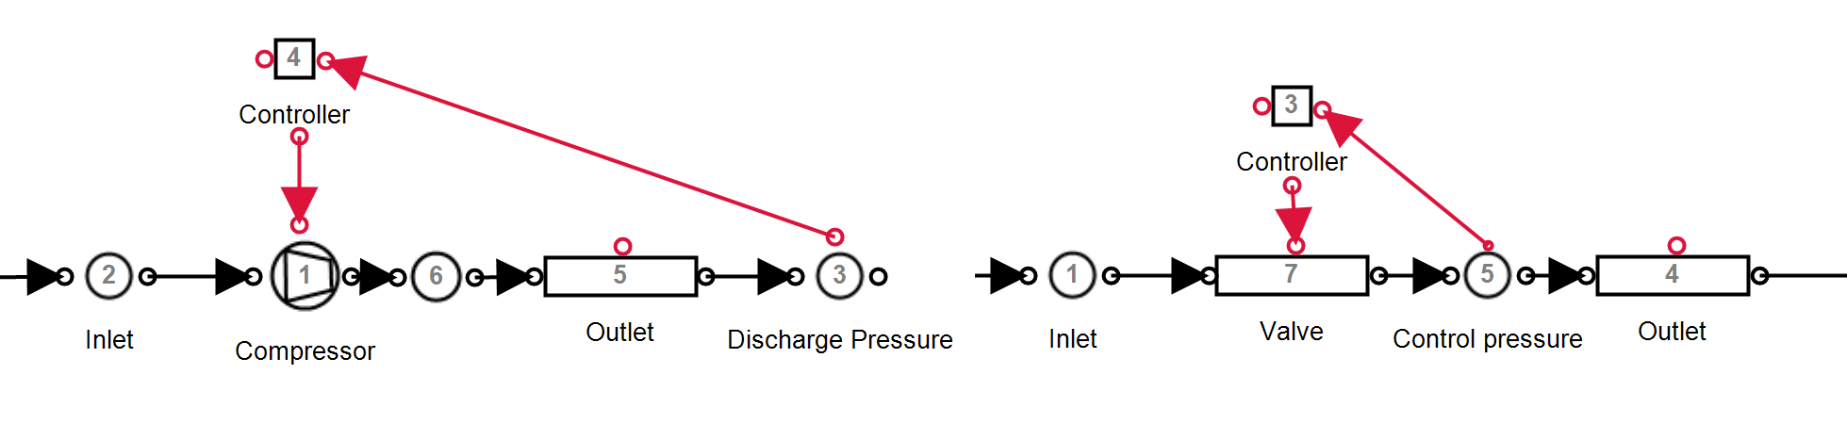
\includegraphics[trim =-4cm 0 -4cm 0cm, width=\textwidth]{Images/3/Controller}}
		\caption{Control components in \gls{stb}.}
		\label{fig: Controller models}
	\end{figure}
		A guide vain controller is developed a \gls{pi} controller as with the \gls{vsd}. However the control limitations of guide vain control, as shown in figure \ref{fig: Guide vain position}, must be added to the model. Figure \ref{fig: Guide vain position} also shows that the typical minimum guide vain control position of 40\% will map to a output power of approx. 60\% of the maximum output power of the compressor.
		\subsubsection{After Cooling}
	\subsection{Simulation inputs}
		-Discuss inputs of the simulation, (compressor setpoints, ambient conditions, demands)
	\subsection{Verification of simulation model}
		- Steps to validate  the model accuracy .\\
		- Compare parameters to actuals
	\subsection{Summary}
\section{Implementation of simulation method}
	\subsection{Preamble}
		Once a model has been developed and verified, the implementation of simulated interventions and scenarios follows. In this section, the approach of implementation, and analysis of interventions in simulation will be discussed.
	\subsection{Analyses of data}
		- Baseline vs Optimised comparison \\
	\subsection{Quantifying operational improvements}
		- Estimating cost savings
	\subsection{Summary}
\section{Conclusion}
